\documentclass[12pt]{article}
\usepackage{ragged2e} 
\usepackage{hyperref}
\usepackage[T1]{fontenc}

\hypersetup{
    colorlinks=true,
    linkcolor=orange!80!black,
    urlcolor=blue,  
    citecolor=blue, 
}

\usepackage[utf8]{inputenc}

\usepackage{pgfplots}
\usepackage{tikz}
\usepackage{pgf-pie}
\usetikzlibrary{pgfplots.statistics}

\usepackage{filecontents}
\usepackage{multirow}
\usepackage{amsmath}
\pgfplotsset{width=10cm,compat=1.17}
\setlength{\parskip}{0.75em} % Spacing between paragraphs
\usepackage{setspace}
\setstretch{1.2} % Adjust the value as per preference
\usepackage[margin=2cm]{geometry} % Adjust the margin
\setlength{\parindent}{0pt} % Adjust value for starting paragraph

\usepackage{mdframed}
\usepackage{float}

\usepackage{xcolor}
\usepackage{titlesec}
\usepackage{titletoc}
\usepackage{listings}
\usepackage{tcolorbox}
\usepackage{lipsum} % Example text package
\usepackage{fancyhdr} % Package for customizing headers and footers

% Define the orange color RGB
\definecolor{myorange}{RGB}{255,65,0}
% Define a new color for "cherry" (dark red)
\definecolor{cherry}{RGB}{148,0,25}
\definecolor{codegreen}{rgb}{0,0.6,0}

%%%%%%%%%%%%%%%%%%%%%%%%%%%%%%%%%%%%%%%%%%%%%%%%%%%%%%%%%%%%%%%%%%%%%
% Apply the custom footer to each page
\fancyhf{} % Clear all header and footer fields
\renewcommand{\headrulewidth}{0pt} % Remove header rule

%%%%%%%%%%%%%%%%%%%%%%%%%%%%%%%%%%%%%%%%%%%%%%%%%%%%%%%%%%%%%%%%%%%%%

% Set the color for the section headings
\titleformat{\section}
{\normalfont\Large\bfseries\color{orange!80!black}}{\thesection}{1em}{}

% Set color for the subsection headings
\titleformat{\subsection}
{\normalfont\large\bfseries\color{orange!80!black}}{\thesubsection}{1em}{}

% Set color for the subsubsection headings
\titleformat{\subsubsection}
{\normalfont\normalsize\bfseries\color{orange!80!black}}{\thesubsubsection}{1em}{}

%%%%%%%%%%%%%%%%%%%%%%%%%%%%%%%%%%%%%%%%%%%%%%%%%%%%%%%%%%%%%%%%%%%%%
% Set color for the table of contents
\titlecontents{section}
[1.5em]{\color{orange!80!black}}
{\contentslabel{1.5em}}
{}{\titlerule*[0.5pc]{.}\contentspage}

% Set the color for the subsections in the table of contents
\titlecontents{subsection}
[3.8em]{\color{orange!80!black}}
{\contentslabel{2.3em}}
{}{\titlerule*[0.5pc]{.}\contentspage}

% Set the color for the subsubsections in the table of contents
\titlecontents{subsubsection}
[6em]{\color{orange!80!black}}
{\contentslabel{3em}}
{}{\titlerule*[0.5pc]{.}\contentspage}

%%%%%%%%%%%%%%%%%%%%%%%%%%%%%%%%%%%%%%%%%%%%%%%%%%%%%%%%%%%%%%%%%%%%%
% set a format for C Code format
\lstset{
    language=C,
    basicstyle=\ttfamily,
    backgroundcolor=\color{blue!5},
    keywordstyle=\color{blue},
    commentstyle=\color{codegreen},
    stringstyle=\color{red},
    showstringspaces=false,
    breaklines=true,
    frame=single,
    rulecolor=\color{lightgray!35}, % Set the color of the frame
    numbers=none,
    numberstyle=\tiny,
    numbersep=5pt,
    tabsize=1,
    alsoletter={\#},
    otherkeywords={\#}
}

\lstdefinestyle{latexstyle}{
    language={[LaTeX]TeX},
    basicstyle=\ttfamily,
    backgroundcolor=\color{blue!5},
    keywordstyle=\color{blue},
    commentstyle=\color{codegreen},
    stringstyle=\color{red},
    showstringspaces=false,
    breaklines=true,
    frame=single,
    rulecolor=\color{lightgray!35}, % Set the color of the frame
    numbers=none,
    numberstyle=\tiny,
    numbersep=5pt,
    tabsize=1,
    morekeywords={documentclass, usepackage, begin, end},
}

% Define a command for inline code snippets with a colored and rounded box
\newtcbox{\codebox}[1][gray]{on line, boxrule=0.2pt, colback=blue!5, colframe=#1, fontupper=\color{cherry}\ttfamily, arc=2pt, boxsep=0pt, left=2pt, right=2pt, top=3pt, bottom=2pt}

%%%%%%%%%%%%%%%%%%%%%%%%%%%%%%%%%%%%%%%%%%%%%%%%%%%%%%%%%%%%%%%%%%%%%

% Define a new tcolorbox style with default options for sections called Tips!
\tcbset{
    myboxstyle/.style={
        colback=orange!10,
        colframe=orange!80!black,
    }
}

% Define a new tcolorbox style with default options to print the output with terminal style
\tcbset{
    myboxstyleTerminal/.style={
        colback=blue!5,
        frame empty, % Set frame to empty to remove the fram
    }
}

\mdfdefinestyle{myboxstyleTerminal1}{
    backgroundcolor=blue!5,
    hidealllines=true, % Remove all lines (frame)
    leftline=false,     % Add a left line
}

\title{ \\ \Large \textbf{Race Car Project}}
\author{George Ghiugan}
\date{January 30, 2023}

\begin{document}
%%%%%%%%%%%%%%%%%%%%%%%%%%%%%%%%%%%%%%%%%%%%%%%%%%%%%%%%%%%%%%%%%%%%%%%%%%%%%%%%%%%%%%%%%%%%%%%%%%%%%%%%%%%%%%%%%%%%%%%%%%%%%%%%%%
\maketitle

\begin{figure}[H]
    \centering
    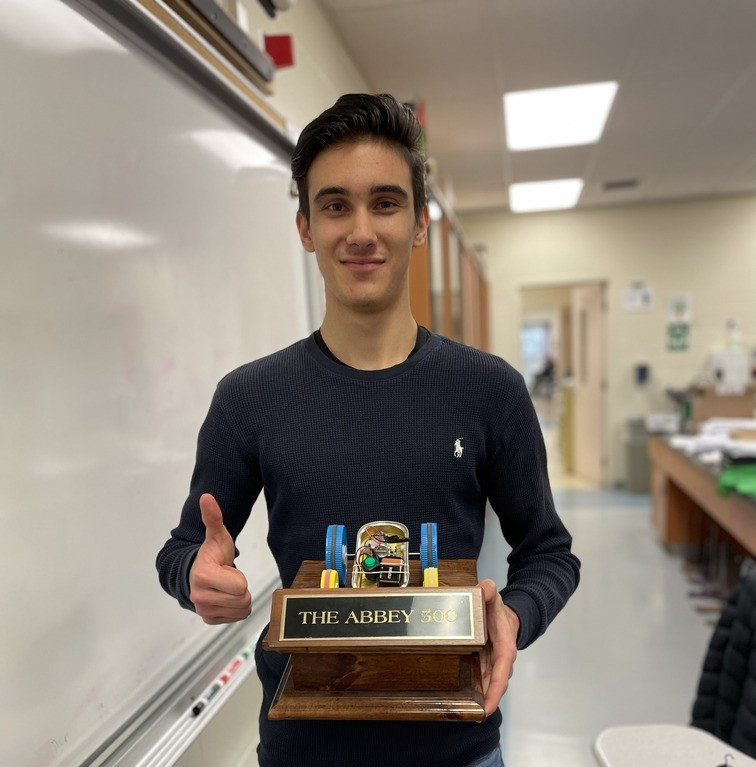
\includegraphics[width=0.7\linewidth]{IMG_5462.jpg}
    \caption{"The Abbey 500" Podium with my first place car design}
    \label{fig:enter-label}
\end{figure}

\section*{Description:}

The purpose of the project was to design a sustainable and functional race car using any available objects and materials necessary. The whole idea of the design was to not use any pre-built car components and to create the fastest car. The only provided materials were the small motor and gears needed for the movement of the car. With this in mind I creatively designed a fast and efficient race car from a tin can resulting in me winning first place in the competition as well as the “Abbey 500” award.

\section*{ Design Process:}

\begin{figure}[H]
    \centering
    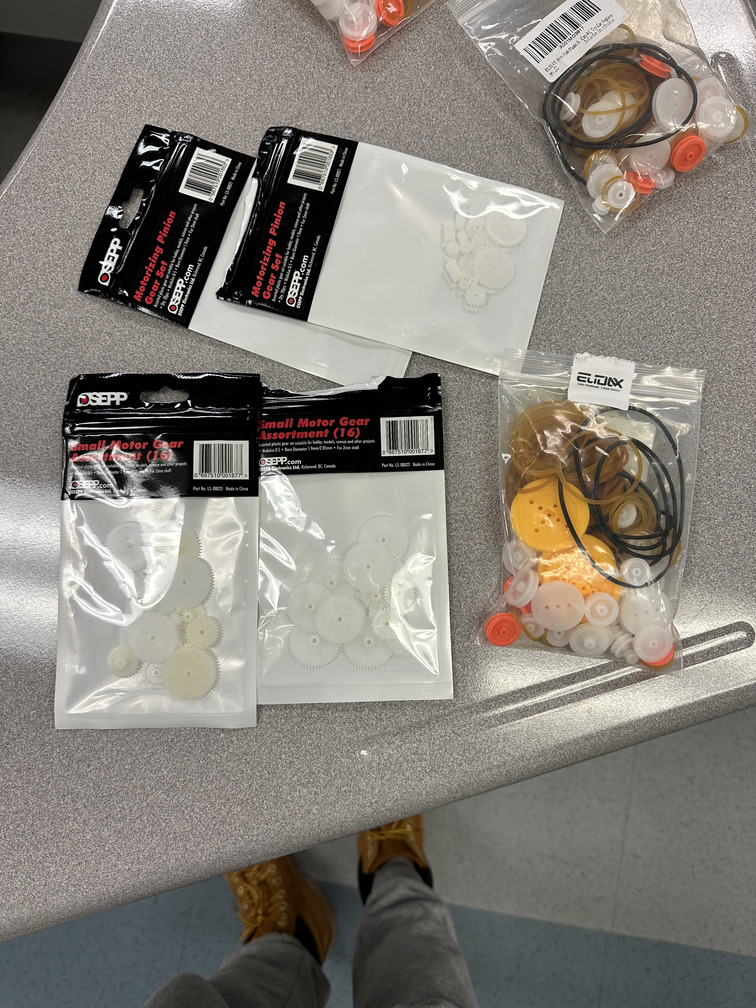
\includegraphics[width=0.5\linewidth]{IMG_0126.jpg}
    \caption{Provided gears and materials}
    \label{fig:enter-label}
\end{figure}

\begin{itemize}
    \item The gears, motors, and elastic bands were provided
  \end{itemize}

\begin{figure}[H]
    \centering
    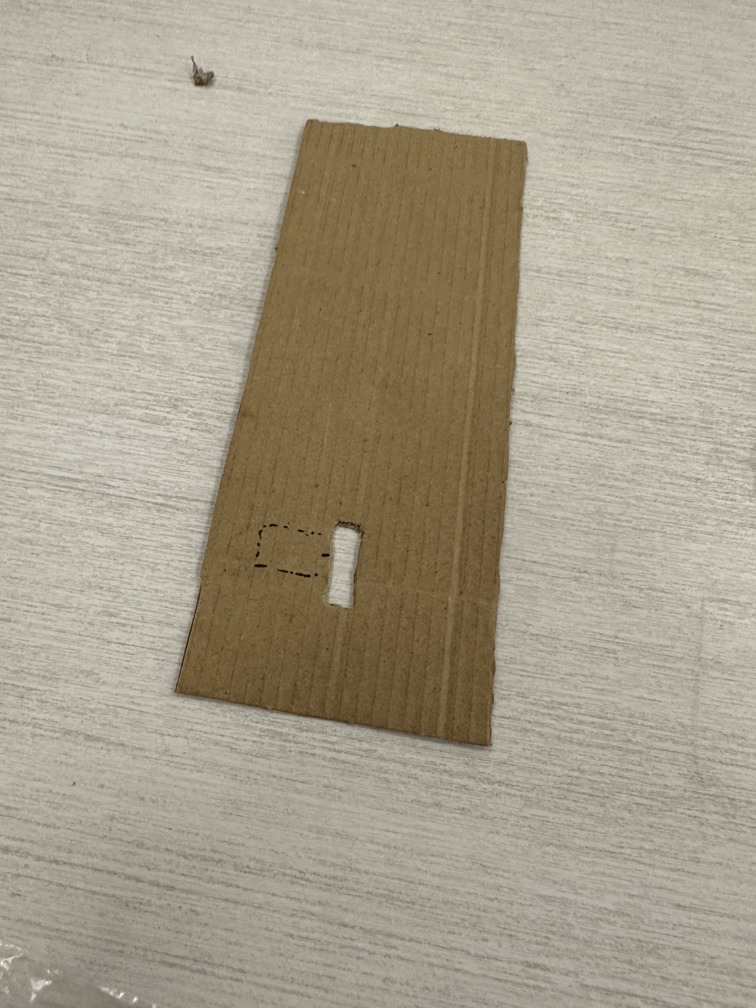
\includegraphics[width=0.5\linewidth]{IMG_0183.jpg}
    \caption{Initial Prototype}
    \label{fig:enter-label}
\end{figure}



\begin{itemize}
    \item This was the initial prototype for the body of the car
    \item Realized that there needed to be a more rigid structure to support the weight of motor, gears, and battery
    \item Decided to use a metal tin can as the car's supporting structure
  \end{itemize}


\begin{figure}[H]
    \centering
    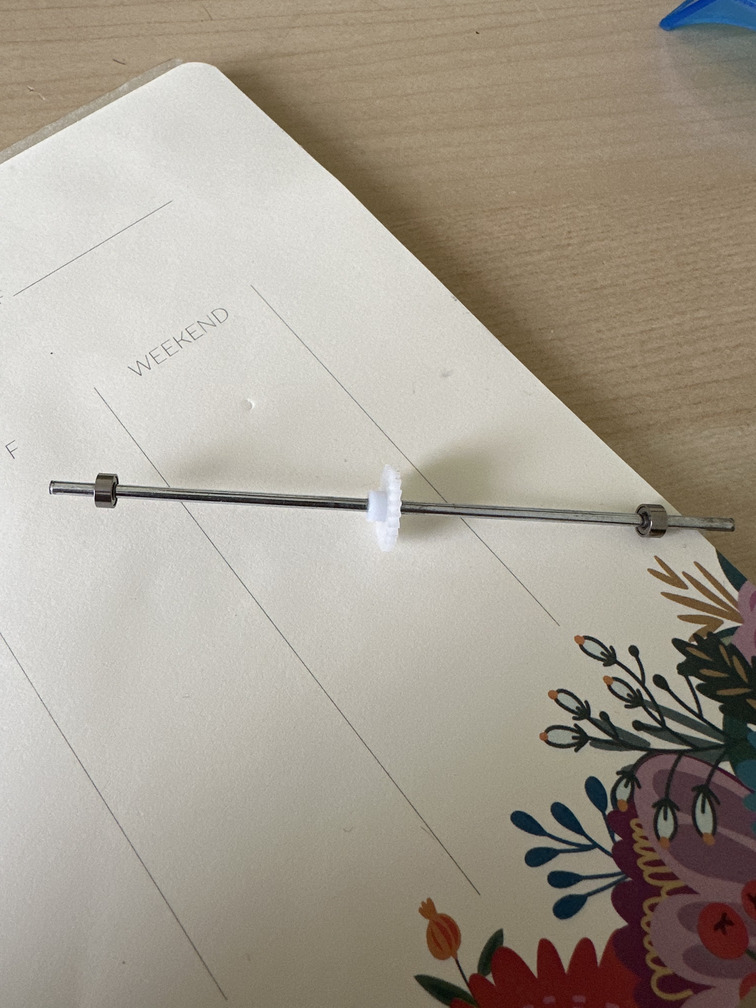
\includegraphics[width=0.7\linewidth]{IMG_0121.jpg}
    \caption{ Adjusting Axle, Bearing, and gear pin}
    \label{fig:enter-label}
\end{figure}

\begin{itemize}
    \item Used axle configuration on bearings allowing for optimal wheel movement at high speeds
    \item Bearings allow for minimal resistance on axle for the fastest and most effective design
    \item Inserted a gear pin in the middle which will allow the motor to transfer rotational power directly to the axle and make the car move
  \end{itemize}


\begin{figure}[H]
    \centering
    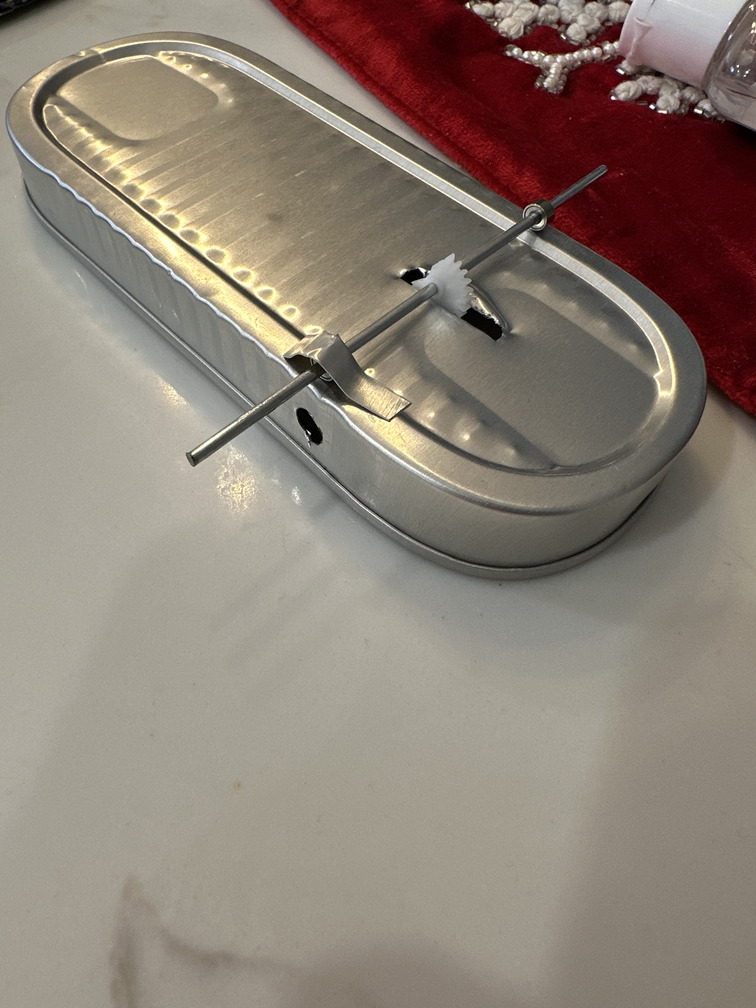
\includegraphics[width=0.7\linewidth]{IMG_0122.jpg}
    \caption{Initial configuration of axle onto the metal body of the car}
    \label{fig:enter-label}
\end{figure}

\begin{itemize}
    \item Cut a hole at the back of the car to allow space for axle to fit with the gear
    \item Secured the bearings onto car structure by gluing a thin piece of metal on top of the bearing
    \item Decided it would be best to shift the gear closer to one side to accomodate the space for the motor
  \end{itemize}


\begin{figure}[H]
    \centering
    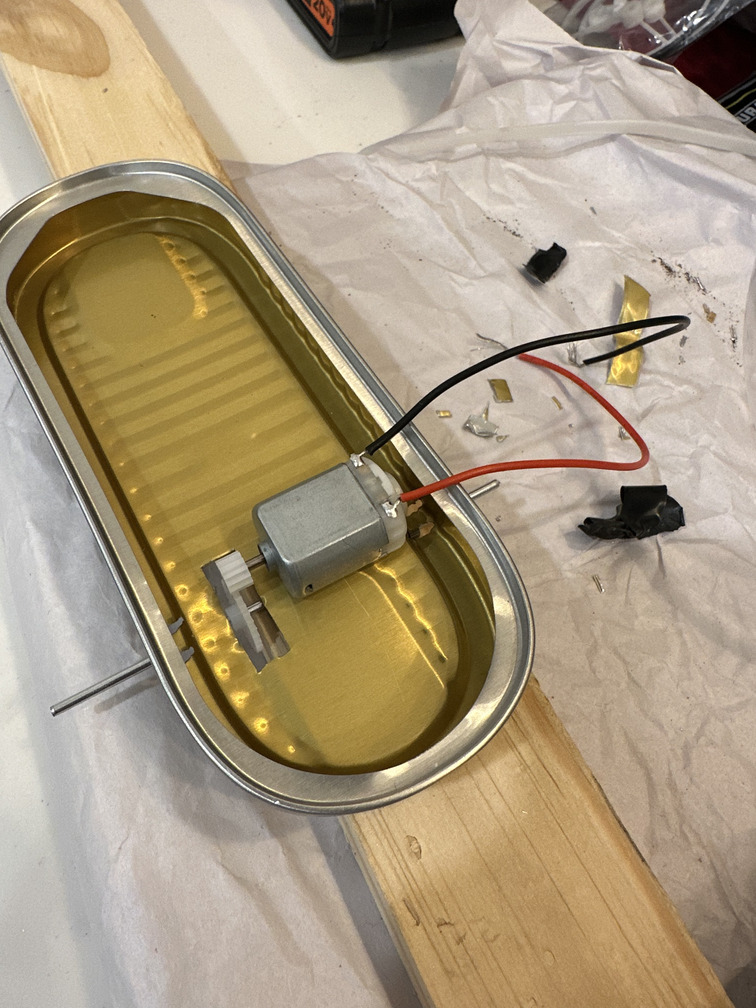
\includegraphics[width=0.7\linewidth]{IMG_0123.jpg}
    \caption{Motor and axle configuration onto the car's body}
    \label{fig:enter-label}
\end{figure}

\begin{itemize}
    \item Adjusted the position of the hole to fit the motor onto the car structure
    \item Positioned axle on the bottom
    \item Used small gear on motor and large gear on the axle for optimal torque and speed 
  \end{itemize}

\begin{figure}[H]
    \centering
    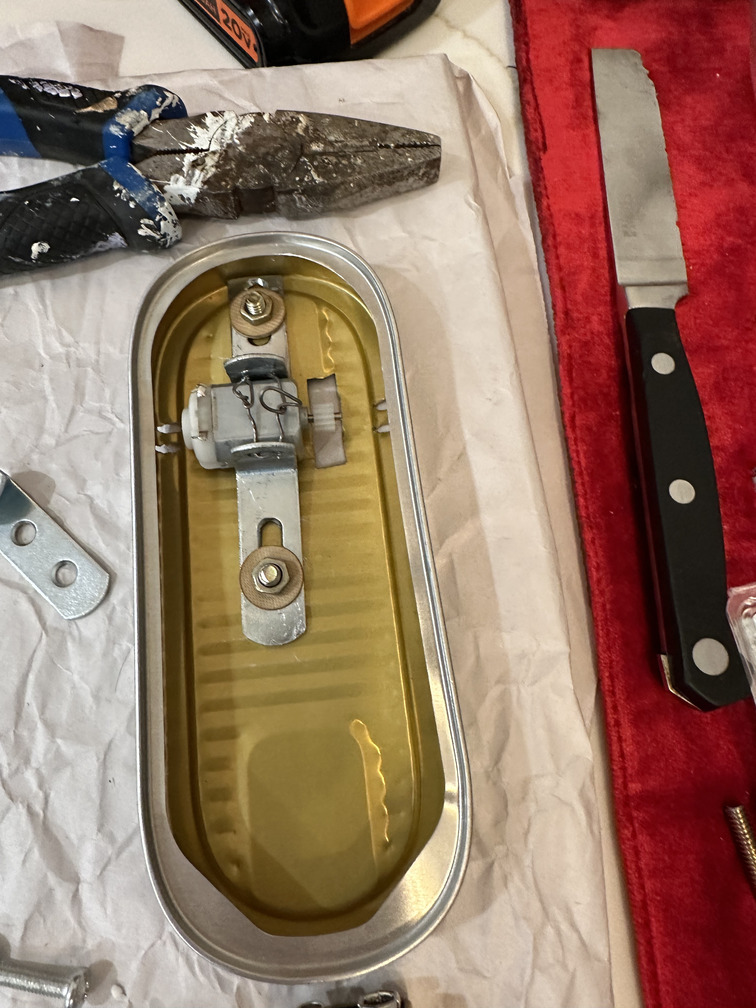
\includegraphics[width=0.7\linewidth]{IMG_0268.jpg}
    \caption{Securing the motor to the body of car}
    \label{fig:enter-label}
\end{figure}

\begin{itemize}
    \item Secured the motor by adding two metal strips to each side
    \item Added screws to firmly secure metal strips and wires on top of motor
    \item Cut two thin slits on each side of motor where the bearings of the axle will be attached with zip-ties
  \end{itemize}


\begin{figure}[H]
    \centering
    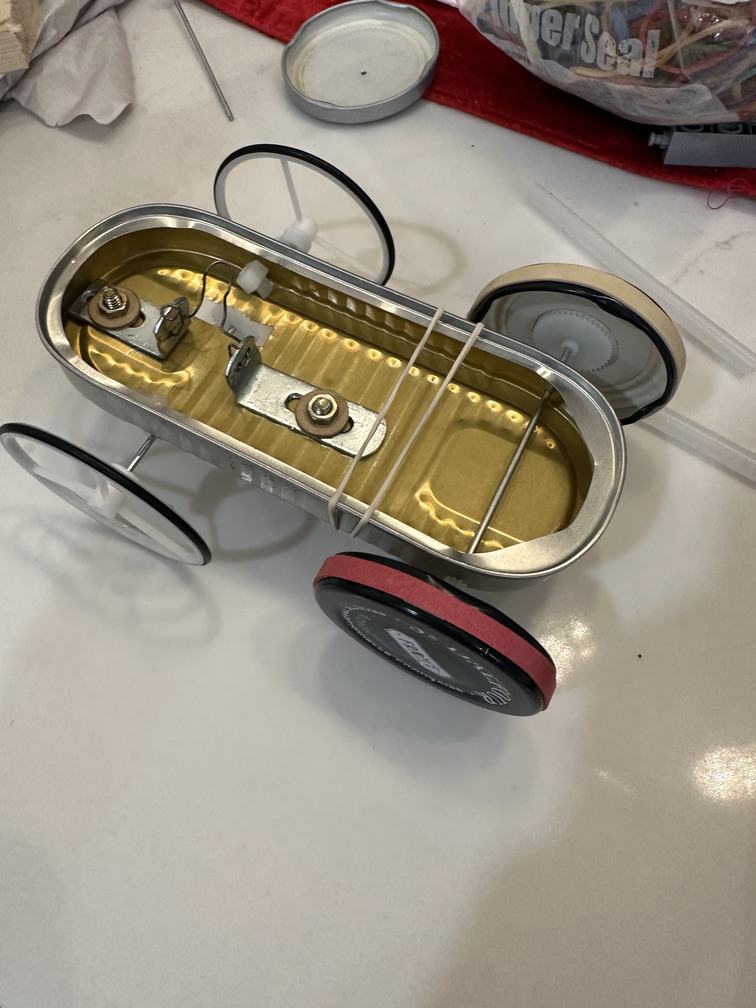
\includegraphics[width=0.7\linewidth]{IMG_0296.jpg}
    \caption{Initial wheel design}
    \label{fig:enter-label}
\end{figure}

\begin{itemize}
    \item Used some cans from jars as the initial wheels
    \item Added elastics for added traction
    \item Drilled two holes on the side of the car in order to slide the axle for the front wheels
    
  \end{itemize}


\begin{figure}[H]
    \centering
    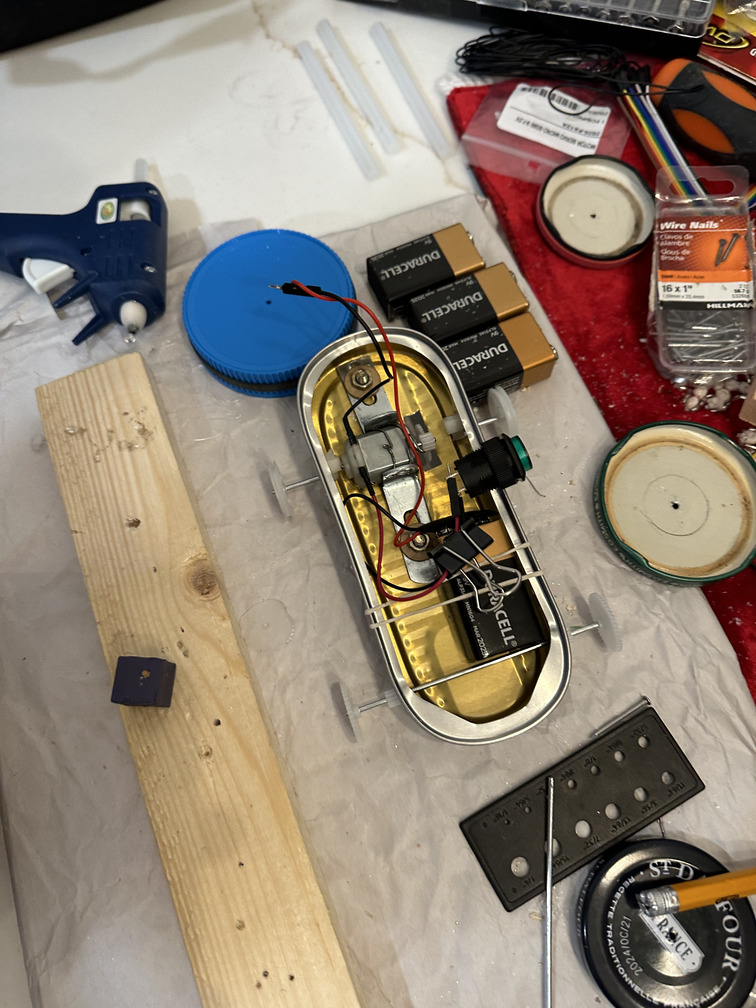
\includegraphics[width=0.7\linewidth]{IMG_0332.jpg}
    \caption{Finalizing car interior}
    \label{fig:enter-label}
\end{figure}

\begin{itemize}
    \item Finishing up the interior of the car with all the required components 
    \item Connecting the 9 volt battery with the motor and setting up push button to start/stop the car
    \item Taped the connecting wires for added reliability
    
  \end{itemize}


\begin{figure}[H]
    \centering
    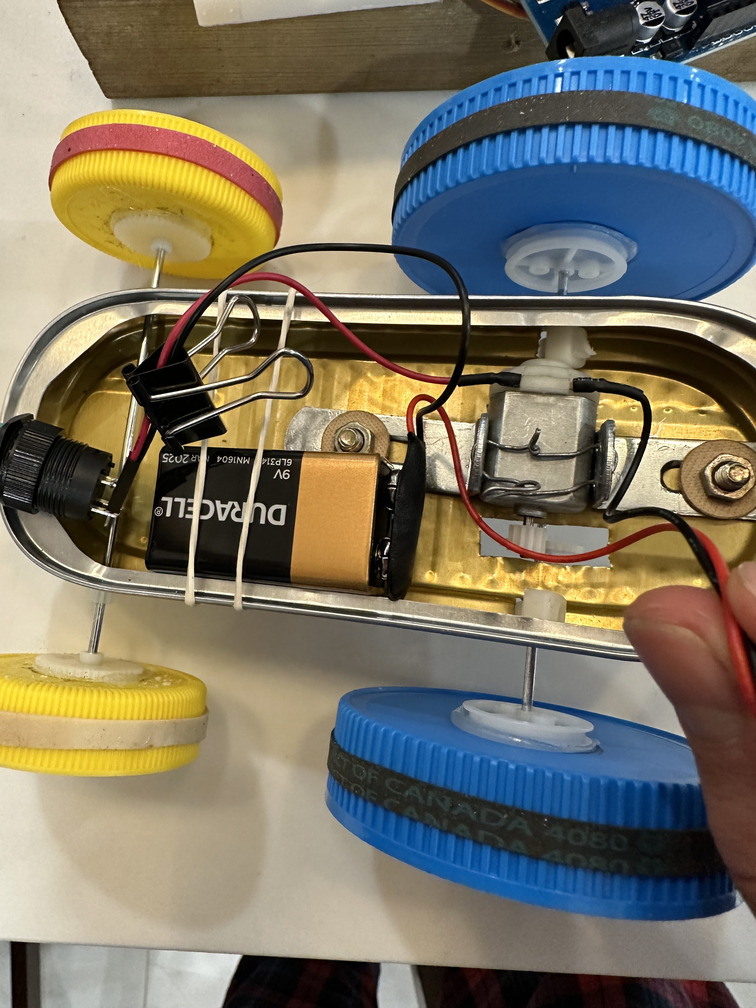
\includegraphics[width=0.7\linewidth]{IMG_0345.jpg}
    \caption{Adding final wheels to the car}
    \label{fig:enter-label}
\end{figure}

\begin{itemize}
    \item After initial prototype of wheels, decided to use lighter plastic lids as the wheels
    \item Larger wheels at the back and smaller ones at the front was the best tested design for wheel configuration
    \item Added rubber elastic bands on each wheel for better traction
    
  \end{itemize}


\begin{figure}[H]
    \centering
    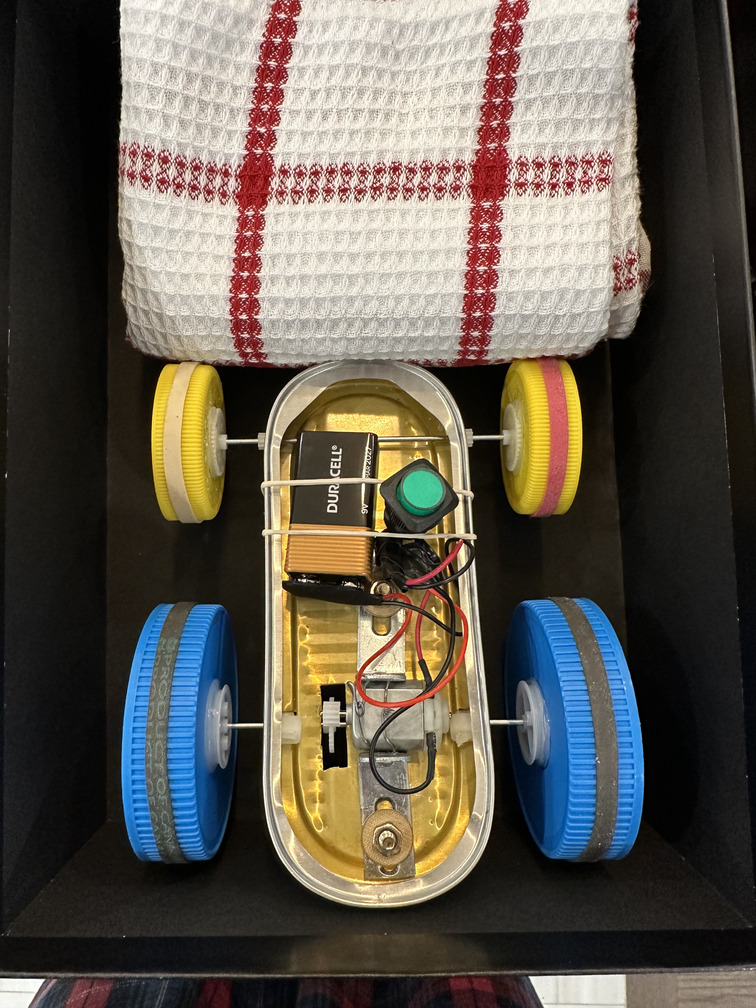
\includegraphics[width=0.7\linewidth]{IMG_0347.jpg}
    \caption{Final Car Design}
    \label{fig:enter-label}
\end{figure}

\begin{itemize}
    \item Top view of the final car design used in the competition
    
  \end{itemize}


\begin{figure}[H]
    \centering
    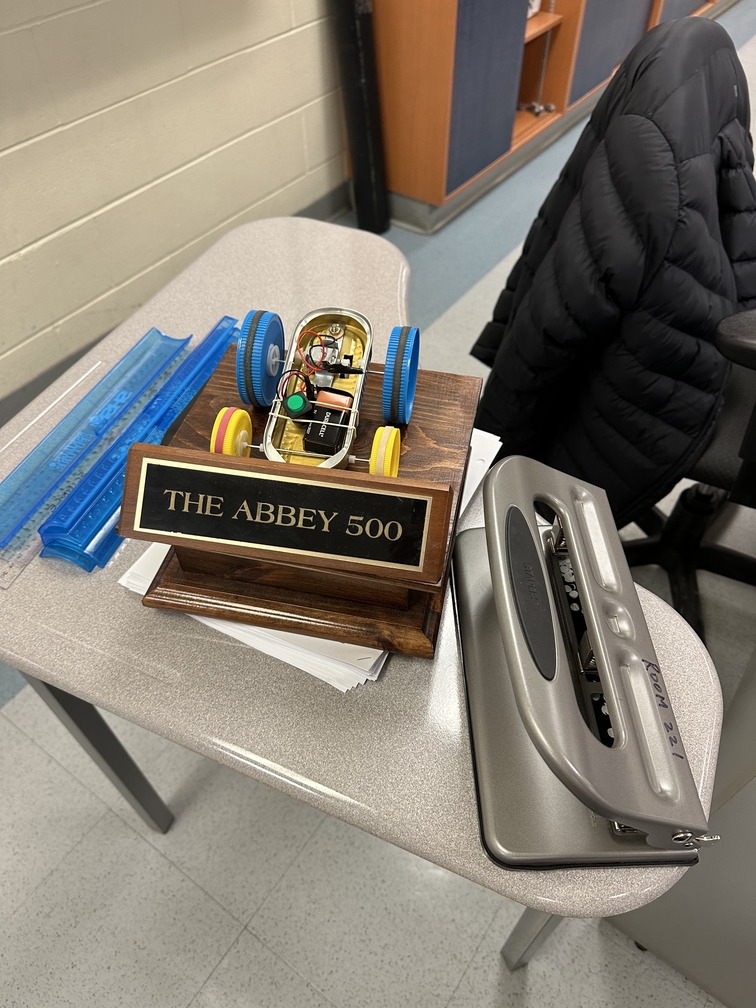
\includegraphics[width=0.7\linewidth]{IMG_0349.jpg}
    \caption{"The Abbey 500" - First Place Podium with race car}
    \label{fig:enter-label}
\end{figure}

\end{document}
